% ==============================================================================
% PAGE 24: 9) PUSH BUTTONS (Numbered Page 16)
% ==============================================================================
\subsubsection*{9) PUSH BUTTONS}

\begin{center}
  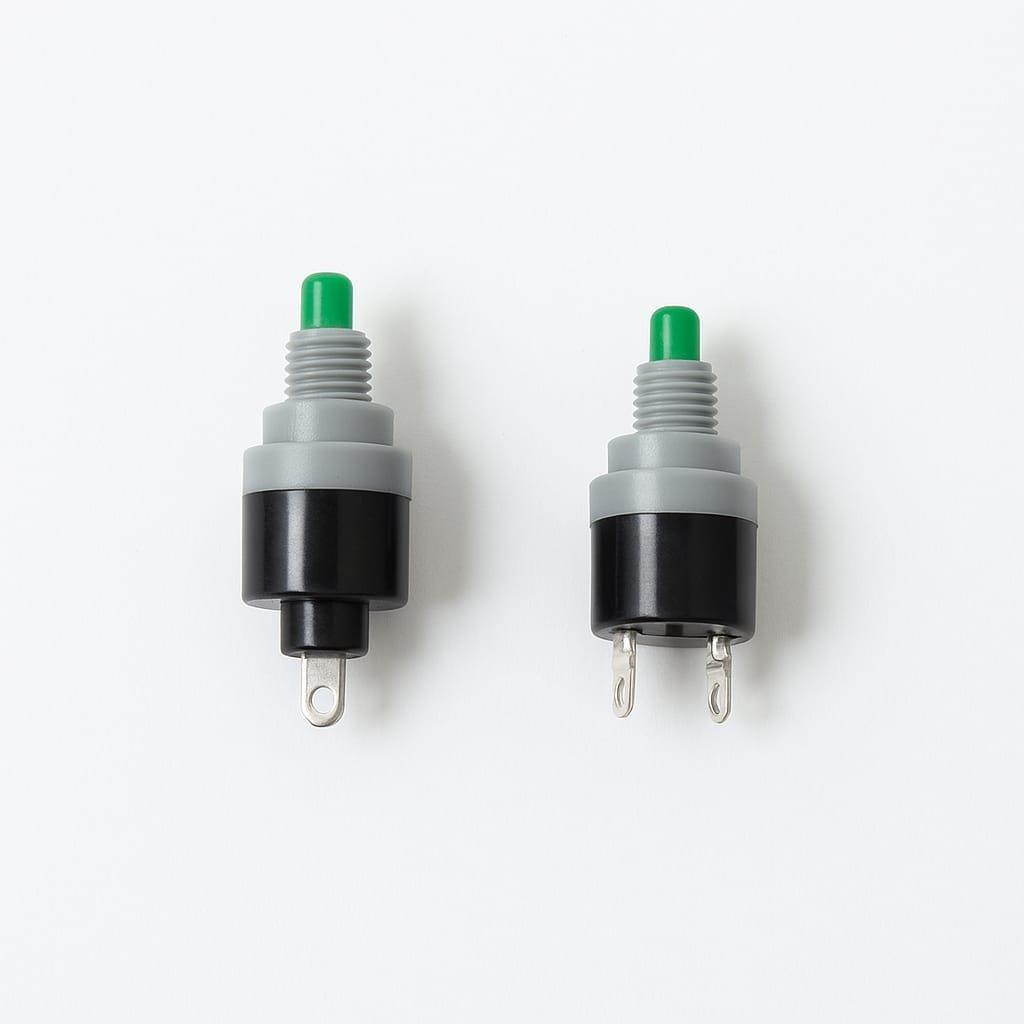
\includegraphics[width=65mm]{figures/fig9_push_buttons.jpg}
\end{center}

\noindent
\begin{spacing}{1.2}
{\fontsize{10.2}{14.5}\selectfont
Push button switches are used as control inputs to operate the motor's direction of rotation. These push buttons are simple, momentary-type switches that make or break an electrical connection when pressed. They are compact, easy to use, and reliable for controlling electronic circuits. Each button is connected to the control pins of the motor driver circuit, which in turn determines the motor's movement direction.\\[3.5mm]
\textbf{Function:}
\begin{itemize}[leftmargin=8mm, itemsep=2mm, label=\textbullet]
  \item There are two push buttons used in the project --- one for right (forward) rotation and the other for left (reverse) rotation of the PMDC motor.
  \item When the right push button is pressed, it sends a signal to the motor driver to rotate the motor in the forward direction.
  \item Similarly, pressing the left push button changes the signal polarity through the driver, causing the motor to rotate in the reverse direction.
  \item Once the button is released, the circuit opens, and the motor stops.
  \item This simple push button control allows easy and manual direction control of the motor.
\end{itemize}
}
\end{spacing}
\clearpage
